\begin{figure}
    \centering
    \begin{minipage}{.5\textwidth}
        \centering
        \begin{tikzpicture}
            \begin{axis}[
                title={\textcolor{blue}{Retain}}, % Add a title to the chart
                xlabel={word a},
                ylabel={word b},
                width=0.75\textwidth, % Adjust the width as needed
                height=0.2\textheight, % Adjust the height as needed
                xmin=1, xmax=5,
                ymin=2, ymax=10,
                legend pos=north west,
                legend entries={$r=1.0$}, % Specify the legend entry
                grid=both,
                ]

                \addplot[
                color=blue,
                mark=*,
                very thick,
                smooth
                ]
                coordinates {
                    (1,2)
                    (2,4)
                    (3,6)
                    (4,8)
                    (5,10)
                };
            \end{axis}
        \end{tikzpicture}
    \end{minipage}%
    %
    \begin{minipage}{.5\textwidth}
        \centering
        \begin{tikzpicture}
        \begin{axis}[
            title={\textcolor{blue}{Retain}}, % Add a title to the chart
            xlabel={word a},
            ylabel={word b},
            width=0.75\textwidth, % Adjust the width as needed
            height=0.2\textheight, % Adjust the height as needed
            xmin=1, xmax=5,
            ymin=1, ymax=5,
            legend pos=north east,
                    legend entries={$r=-1.0$}, % Specify the legend entry
            grid=both,
        ]

        \addplot[
            color=red,
            mark=square,
                very thick,
            smooth
            ]
            coordinates {
                (5,1)
                (4,2)
                (3,3)
                (2,4)
                (1,5)
            };
        \end{axis}
            \end{tikzpicture}
        \end{minipage}%

        %\rule{\textwidth}{1pt}
        \bigskip
    \begin{minipage}{.5\textwidth}
        \centering
        \begin{tikzpicture}
        \begin{axis}[
            title={\textcolor{blue}{Retain}}, % Add a title to the chart
            xlabel={word a},
            ylabel={word b},
            width=0.75\textwidth, % Adjust the width as needed
            height=0.2\textheight, % Adjust the height as needed
            xmin=1, xmax=5,
            ymin=2, ymax=10,
            legend pos=north west,
                    legend entries={$r=.66$}, % Specify the legend entry
            grid=both,
        ]

        \addplot[
            color=purple,
            mark=o,
            very thick,
            smooth
            ]
            coordinates {
                (1,3)
                (2,2.2)
                (3,5)
                (4,2.2)
                (5,10)
            };
        \end{axis}
        \end{tikzpicture}
    \end{minipage}%
    %
    \begin{minipage}{.5\textwidth}
        \centering
        \begin{tikzpicture}
        \begin{axis}[
            title={\textcolor{red}{Drop}}, % Add a title to the chart
            xlabel={word a},
            ylabel={word b},
            width=0.75\textwidth, % Adjust the width as needed
            height=0.2\textheight, % Adjust the height as needed
            xmin=1, xmax=5,
            ymin=2, ymax=10,
            legend pos=north west,
                legend entries={$r=.37$}, % Specify the legend entry
            grid=both,
        ]

        \addplot[
            color=orange,
            mark=diamond,
                very thick,
            smooth
            ]
            coordinates {
                (1,6)
                (2,2.5)
                (3,6)
                (4,2.5)
                (5,10)
            };
        \end{axis}
        \end{tikzpicture}
    \end{minipage}
    \caption{Lexical variables selection by correlation}
    \label{fig:lexical_variables_selection_by_correlation}
\end{figure}
